\subsection{Task1.3-spatial and body form for product of exponential}
%\subsubsection{Task1.3 Power of Exponentials formulations}
\label{title:Task1.3}

%product of exponentials (PoE)
%important knowlege:
%what is a screw axis?
%-> a matrix of repesenting the linear velocity v and angular velocity $\omega$
%-> is essencial to build the exponential coordinats ==> $S \theta$ 
%-> analogous to $\omega$ axis (P98 in Book)
%-> can be expressed in SE(3) 

In forward kinematics an open-chain manipulator can be described with the product of exponential (PoE) in spatial form \ref{eq:spatial_form} or in body form\ref{eq:body_form}.  
\begin{align}\label{eq:spatial_form}
    T_S(\theta) = e^{[S_1]\theta_1} ... e^{[S_n-1]\theta_n-1} e^{[S_n]\theta_n} M 
\end{align} 
\begin{equation}\label{eq:body_form}
    T_B(\theta) = M e^{[B_1]\theta_1} ... e^{[B_n-1]\theta_n-1} e^{[B_n]\theta_n}
\end{equation}
The difference between the equations is, witch reference frame was chosen .  \\
The figure \ref{fig:openchain} shows an example for an open chain robot. On the basis of it the theoretical equations will be explained. The requirements to bulit a PoE are 
\begin{itemize}
    \item a body and a space frame,
    \item to set the robot in its zero position and
    \item to know all the joint variables $\theta$.
\end{itemize}
\begin{figure}[H]
    \centering
    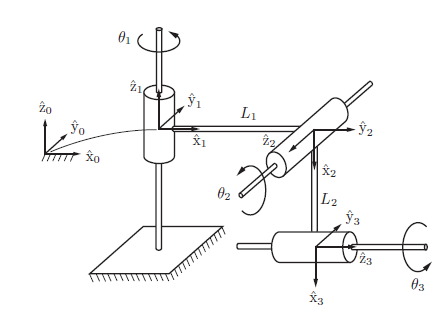
\includegraphics[width=0.5\textwidth]{Images/Task1.3/task1.3_openchain.PNG}
    \caption[]{A 3R spatial open chain in its home position.}
    \label{fig:openchain}
    \source{book P 143}
\end{figure}

The first step of the PoE is to determine the end-effector matrix M. This matrix represent the relation from the space frame to the body frame in the robots zero position, also called home position. This matrix is the same for the space and the body form of PoE. In other words M is the transformation matrix $T_{sb}$ for the home position. \\
In addition it is interesting to noticed that M, in the equation \ref{eq:spatial_form} and \ref{eq:body_form} is connected to the least significant joint, or rather the most far away joint from the consider frame. In words it means that for the spacial form M is calculated first with the joint n and in the body form M is multiplied by the first joint. 
\begin{equation}
    M = 
    \begin{bmatrix}
        0 & 0 & 1 & L_1\\
        0 & 1 & 0 & 0 \\
        -1 & 0 & 0 &-L_2\\
        0 & 0 & 0 & 1
    \end{bmatrix}
\end{equation}
The next step is to write down the screw axis for every joint. We start with the \textbf{spacial form}. As a reminder of how screw axis can look like, the figure\ref{fig:screw_axis} is added.  For the PoE it is mandatory to use the SE(3) form of the screw axes. But in easy terms it can be note in a table like in \ref{tab:screwS}. The values for $\omega$ can be read out of the picture. The values of  the linear velocity $v$ are made by $v_n =  -\omega_n \times q_n$. Whereat $q_n$ is a point on the $\omega_n$ axes. The i in the variable stays for the joins n for the direction in a frame 1 for x, 2 for y and 3 for z. 
\begin{figure}[H]
    \centering
    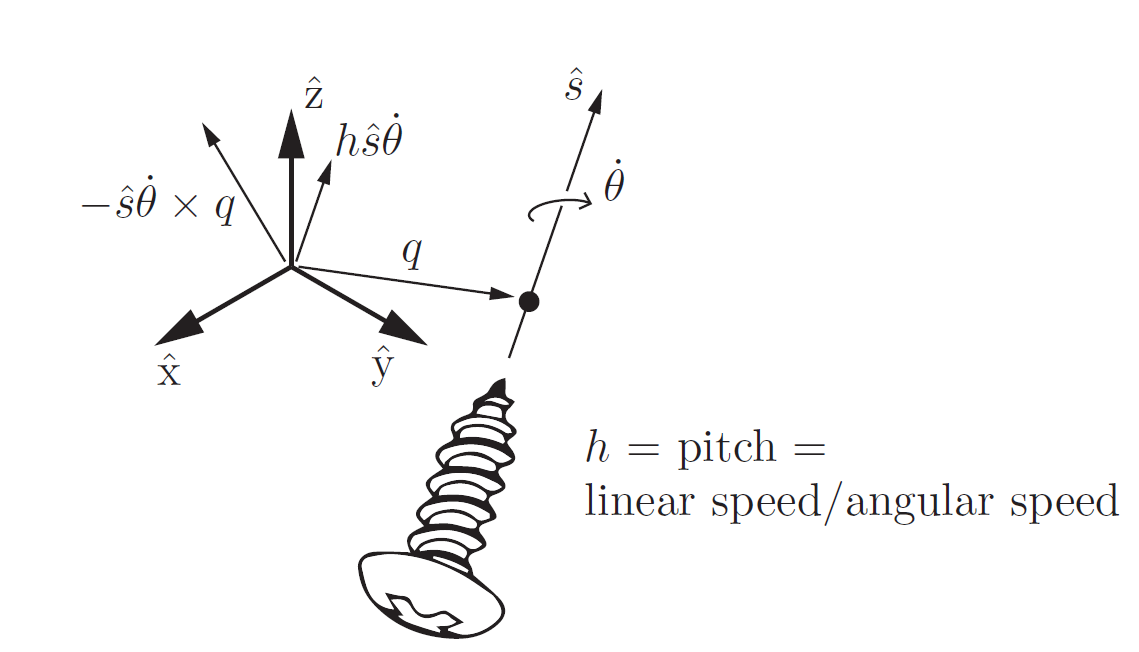
\includegraphics[width=0.5\textwidth]{Images/Task1.3/scew_axis.PNG}
    \caption[screw axis]{A screw axis S represented by a point q, a unit direction s, and a pitch.}
    \label{fig:screw_axis}
    %\source{Insert image source here}
\end{figure}

\begin{equation} \label{eq:S}
    [S] =
    \begin{bmatrix}
        [\omega] &  v \\
        0 & 0
    \end{bmatrix} 
     = 
    \begin{bmatrix}
        0 & -\omega_{i3} & \omega_{i2} & -\omega_{in} \times q_{in}\\
        \omega_{i3} & 0 & -\omega_{i1} & -\omega_{in} \times q_{in}\\
        -\omega_{i2} & \omega_{i1} & 0& -\omega_{in} \times q_{in}\\
        0 & 0 & 0 & 0\\
        \end{bmatrix}
	\end{equation}

\begin{table}[h] 
    \centering
    \begin{tabular}{c||c|c}
         i & $\omega_i$ & $v_i$\\
         \hline
         1 & (0,0,1) & (0,0,0)\\
         \hline
         2 & (0,-1,0) & (0,0,$L_1$)\\
         \hline
         3 & (1,0,0) & (0,$L_2$,0)\\
    \end{tabular}
    \caption{screw axes $S_i$}
    \label{tab:screwS}
\end{table}

%-> figure 3.19 is good for understanding what a screw axis is


The expression for $S$ as a vector is $S_n =
    \begin{bmatrix}
        \omega_n \\
        v_n
    \end{bmatrix}$. But this form is not in use for the PoE. Through the space form, the \textbf{body form} can be transformed.
\begin{align*} \label{eq1:T}
        T(\theta) &= e^{[S_1]\theta_1} ... e^{[S_n]\theta_n} M \\
                  &= e^{[S_1]\theta_1} ... M e^{M^{-1}[S_n] M \theta_n}\\
                  &= e^{[S_1]\theta_1} ... M e^{M^{-1}[S_{n-1}] M \theta_{n-1}} \cdot e^{M^{-1}[S_n] M \theta_n}\\
                  &= M e^{M^{-1}[S_{1}] M \theta_{1}...} e^{M^{-1}[S_{n-1}] M \theta_{n-1}} \cdot e^{M^{-1}[S_{n}] M \theta_{n}}\\
                  &= Me^{[B_1]\theta_1} ... e^{[B_{n-1}]\theta_{n-1}} \cdot e^{[B_n]\theta_n} M
\end{align*}
For the transformation the mathematical rule of equation \ref{eq:BequalS} is used.
\begin{equation}\label{eq:BequalS}
    B_i = M^{-1}[S_{i}] M = [Ad_M^{-1}] S_i
\end{equation}

In general the body form has the same borders as the space form. That means the equation \ref{eq:B} and the table can be used as well. In order to the example the screw axis are presented in table \ref{tab:screwB}. The body frame is the frame with the indices 3.

\begin{equation} \label{eq:B}
    [B] =
    \begin{bmatrix}
        [\omega] &  v \\
        0 & 0
    \end{bmatrix} 
\end{equation}
\begin{table}[h] 
    \centering
    \begin{tabular}{c||c|c}
         i & $\omega_i$ & $v_i$\\
         \hline
         1 & (-1,0,0) & (0,$L_1$,0)\\
         \hline
         2 & (0,-1,0) & (0,0,$L_2$)\\
         \hline
         3 & (1,0,0) & (0,0,0)\\
    \end{tabular}
    \caption{screw axes $B_i$}
    \label{tab:screwB}
\end{table}

In the end the result of $T_S$ and $T_B$ is the same. 
...hmm i don't know how to do it python .... 
but i tryed it and you can see it on github..

%%--------------------------------------------------------------------------
%notes
\begin{comment}
-what are the exponential coordinats?
-> a way to describe points in the space of a robot 
-> 
\par
%main
\textbf{spatial form} \par
In the use of the spatial form, every screw axes is described in relation to the fixed-frame resp. frame{0} of the robot. 
%do I explain it with the exsample in the book ? 
The screw axes can be expressed as
\begin{equation} \label{eq:S_n}
    S_n =
    \begin{bmatrix}
        \omega_n \\
        v_n
    \end{bmatrix}
    \in 
    \mathbb{R}^{1 \times (2*n)}
	\end{equation}
approach:
(chapter 4.1)
-you need:
    -stationary frame {s}
    -end-effector frame {b}
    -zero position of the robot (joint values are zero and direction of positiv displacement
    -all joint variables $\theta_n$
-you make:
    - all $S_n$ (screw axes) expressed in Space frame
    -M matrixes as 'denote the configuration of the TCP frame relaive to the fixed base frame for robot in zero position ' (=home position)
    - equation   \eqref{eq1:TinPoE}
-consider by calulating:
    -revolute joints:
        -$\omega_n $  as unit vector and pos. direction of joint axis n
        -linear velocity is \eqref{eq1:v_n}
        - $q_n$ is point on joint axes (in view of fixed base frame)
        -$\theta$ as joint angle
        \begin{equation} \label{eq1:v_n}
    v_n =  -\omega_n \times q_n 
	\end{equation}
    -prismatic joints:
        -$\omega_n = 0$
        -$v_n$ is unit vector and posi translation 
        -$\theta$ shows prismatic extension/retraction
-result T:
    -shows ne configuration of TCP frame 
    -for varying of $\theta$ just multiply $e^{[S_n]\theta_n}$ ->
    \begin{equation} 
        T(\theta) = (\Pi_{n=1}^N  e^{[S_n]\theta_n}) M 
        \qquad
    	\end{equation}
\par
\textbf{body form} \par
-screw axis is discripte by body  frame -> $B$
-transformation:
\begin{align*} 
        T(\theta) &= (\Pi_{n=1}^N  e^{[S_n]\theta_n}) M \\
                  &= e^{[S_1]\theta_1} ... e^{[S_n]\theta_n} M \\
                  &= e^{[S_1]\theta_1} ... M e^{M^{-1}[S_n] M \theta_n}\\
                  &= e^{[S_1]\theta_1} ... M e^{M^{-1}[S_n] M \theta_n}\\
\end{align*}
-bzw 
\begin{equation}
    B_i = [Ad_M^{-1}] S_i
\end{equation}
-interessting -> place of M in the equations:
    -space form M is first transformed with most distal joint -> Si is unaffected by most distal transformation
    -body from M is first proximal joint -> B unaffected by proximal joint
\begin{equation} \label{eq1:B_n}
    B_n =
    \begin{bmatrix}
        \omega_n \\
        v_n
    \end{bmatrix}
    \in 
    \mathbb{R}^{1 \times (n+n)}
	\end{equation}



-> maybe i will just make a big table 
%conclution
-basicly the exsample of P 141
-maybe with the picture of 141 Product of Exponentials Formula
To use the PoE formula, it is only necessary to assign a stationary frame
% i would not do an example here, we can refer to task 2 for the example
\begin{equation} \label{eq1:TinPoE}
    T = e^{[S_n]\theta_n} M 
	\end{equation}


\end{comment}
